\section{First section}

\begin{frame}
  \frametitle{Things we might want to consider/try}
%
\begin{itemize}
  \item Is it a bug in the frontend (clang) or the backend
    (llvm) that is causing the bug?
    (http://permalink.gmane.org/gmane.comp.compilers.llvm.devel/79491)
  \item Is it possible to trigger similar behaviour with
    other (slightly different?) assertions? Try.
  \item Try and fuzz the compiler ourselves?
  \item Do a complete write-up of how to replicate the bug -
    from installation to obtaining root access through sudo.
  \item Find a (funny?) program and insert the bug.
\end{itemize}
%
\end{frame}



\begin{frame}
  \frametitle{Things we should read}
%
\begin{itemize}
  \item Ken Thompson - Reflections on Trusting Trust.
  \item Maybe this one about the above (haven't read it
    myself): http://wiki.c2.com/?TheKenThompsonHack
  \item The fuzzing-attack on the clang/llvm compiler:
    http://permalink.gmane.org/gmane.comp.compilers.llvm.devel/79491
\end{itemize}
\end{frame}



\begin{frame}
  \frametitle{What are clang and LLVM?}
  %
  \begin{figure}
    \centering
    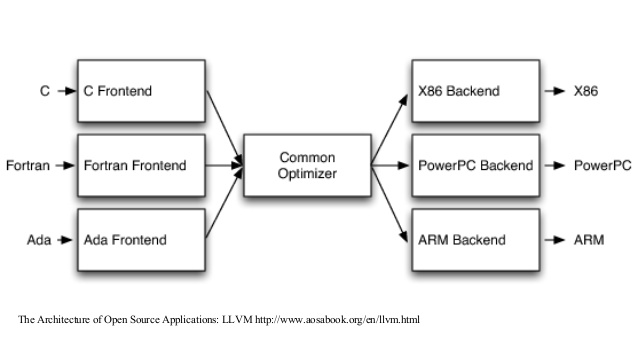
\includegraphics[scale=0.3]{input/content/figures/clang-llvm}
  \end{figure}
%
\begin{description}[short]
  \item[clang] a C language family frontend for LLVM. (http://clang.llvm.org/)
  \item[LLVM] ``The LLVM Core libraries provide a modern
    source- and target-independent optimizer, along with
    code generation support for many popular CPUs.`` (http://llvm.org/)
\end{description}
%
Sidenote: ``The LLVM Project is a collection of modular and
reusable compiler and toolchain technologies.''


\end{frame}
